% ============================================================================
% Model 7: Quantile Regression
% WARNING: RESEARCH ONLY - NOT REGULATORY COMPLIANT
% ============================================================================

\chapter{Model 7: Quantile Regression (Research Only)}
\label{ch:model7}

% Load command values
% Model 7 Calibrated Values
% Generated: 2025-10-07 09:39:44.326058
% Model: Quantile Regression

% Core Metrics
\renewcommand{\ModelSevenRSquaredTrain}{0.2524}
\renewcommand{\ModelSevenRSquaredTest}{0.2246}
\renewcommand{\ModelSevenRMSETrain}{38,160}
\renewcommand{\ModelSevenRMSETest}{38,456}
\renewcommand{\ModelSevenMAETrain}{27,199}
\renewcommand{\ModelSevenMAETest}{27,562}
\renewcommand{\ModelSevenMAPETrain}{84.7}
\renewcommand{\ModelSevenMAPETest}{85.3}
\renewcommand{\ModelSevenCVMean}{0.2516}
\renewcommand{\ModelSevenCVStd}{0.0147}
\renewcommand{\ModelSevenWithinOneK}{3.7}
\renewcommand{\ModelSevenWithinTwoK}{7.0}
\renewcommand{\ModelSevenWithinFiveK}{15.1}
\renewcommand{\ModelSevenWithinTenK}{27.5}
\renewcommand{\ModelSevenWithinTwentyK}{49.1}
\renewcommand{\ModelSevenTrainingSamples}{53,812}
\renewcommand{\ModelSevenTestSamples}{13,453}

% Subgroup Metrics
\renewcommand{\ModelSevenSubgrouplivingFHN}{11,666}
\renewcommand{\ModelSevenSubgrouplivingFHRSquared}{0.228}
\renewcommand{\ModelSevenSubgrouplivingFHRMSE}{39,026}
\renewcommand{\ModelSevenSubgrouplivingFHBias}{-6,165}
\renewcommand{\ModelSevenSubgrouplivingILSLN}{1,787}
\renewcommand{\ModelSevenSubgrouplivingILSLRSquared}{0.199}
\renewcommand{\ModelSevenSubgrouplivingILSLRMSE}{34,506}
\renewcommand{\ModelSevenSubgrouplivingILSLBias}{-3,258}
\renewcommand{\ModelSevenSubgroupageAgeUnderTwentyOneN}{1,300}
\renewcommand{\ModelSevenSubgroupageAgeUnderTwentyOneRSquared}{0.017}
\renewcommand{\ModelSevenSubgroupageAgeUnderTwentyOneRMSE}{40,058}
\renewcommand{\ModelSevenSubgroupageAgeUnderTwentyOneBias}{-14,382}
\renewcommand{\ModelSevenSubgroupageAgeTwentyOneToThirtyN}{3,770}
\renewcommand{\ModelSevenSubgroupageAgeTwentyOneToThirtyRSquared}{0.176}
\renewcommand{\ModelSevenSubgroupageAgeTwentyOneToThirtyRMSE}{43,445}
\renewcommand{\ModelSevenSubgroupageAgeTwentyOneToThirtyBias}{-7,298}
\renewcommand{\ModelSevenSubgroupageAgeThirtyOnePlusN}{8,383}
\renewcommand{\ModelSevenSubgroupageAgeThirtyOnePlusRSquared}{0.259}
\renewcommand{\ModelSevenSubgroupageAgeThirtyOnePlusRMSE}{35,716}
\renewcommand{\ModelSevenSubgroupageAgeThirtyOnePlusBias}{-3,762}
\renewcommand{\ModelSevenSubgroupcostQOneLowN}{3,365}
\renewcommand{\ModelSevenSubgroupcostQOneLowRSquared}{-10.000}
\renewcommand{\ModelSevenSubgroupcostQOneLowRMSE}{33,109}
\renewcommand{\ModelSevenSubgroupcostQOneLowBias}{+25,519}
\renewcommand{\ModelSevenSubgroupcostQTwoN}{3,362}
\renewcommand{\ModelSevenSubgroupcostQTwoRSquared}{-7.118}
\renewcommand{\ModelSevenSubgroupcostQTwoRMSE}{20,447}
\renewcommand{\ModelSevenSubgroupcostQTwoBias}{+10,411}
\renewcommand{\ModelSevenSubgroupcostQThreeN}{3,363}
\renewcommand{\ModelSevenSubgroupcostQThreeRSquared}{-3.662}
\renewcommand{\ModelSevenSubgroupcostQThreeRMSE}{24,857}
\renewcommand{\ModelSevenSubgroupcostQThreeBias}{-12,991}
\renewcommand{\ModelSevenSubgroupcostQFourHighN}{3,363}
\renewcommand{\ModelSevenSubgroupcostQFourHighRSquared}{-2.124}
\renewcommand{\ModelSevenSubgroupcostQFourHighRMSE}{61,508}
\renewcommand{\ModelSevenSubgroupcostQFourHighBias}{-46,070}

% Variance Metrics
\renewcommand{\ModelSevenCVActual}{1.011}
\renewcommand{\ModelSevenCVPredicted}{0.676}
\renewcommand{\ModelSevenPredictionInterval}{149,036}
\renewcommand{\ModelSevenBudgetActualCorr}{0.499}
\renewcommand{\ModelSevenQuarterlyVariance}{88.0}
\renewcommand{\ModelSevenAnnualAdjustmentRate}{92.7}

% Population Scenarios
\renewcommand{\ModelSevenPopcurrentbaselineClients}{32,085}
\renewcommand{\ModelSevenPopcurrentbaselineAvgAlloc}{37,400}
\renewcommand{\ModelSevenPopcurrentbaselineWaitlistChange}{+0}
\renewcommand{\ModelSevenPopcurrentbaselineWaitlistPct}{+0.0}
\renewcommand{\ModelSevenPopmodelbalancedClients}{32,726}
\renewcommand{\ModelSevenPopmodelbalancedAvgAlloc}{36,652}
\renewcommand{\ModelSevenPopmodelbalancedWaitlistChange}{+641}
\renewcommand{\ModelSevenPopmodelbalancedWaitlistPct}{+2.0}
\renewcommand{\ModelSevenPopmodelefficiencyClients}{33,689}
\renewcommand{\ModelSevenPopmodelefficiencyAvgAlloc}{35,530}
\renewcommand{\ModelSevenPopmodelefficiencyWaitlistChange}{+1,604}
\renewcommand{\ModelSevenPopmodelefficiencyWaitlistPct}{+5.0}
\renewcommand{\ModelSevenPopcategoryfocusedClients}{27,272}
\renewcommand{\ModelSevenPopcategoryfocusedAvgAlloc}{44,132}
\renewcommand{\ModelSevenPopcategoryfocusedWaitlistChange}{-4,812}
\renewcommand{\ModelSevenPopcategoryfocusedWaitlistPct}{-15.0}
\renewcommand{\ModelSevenPoppopulationmaximizedClients}{36,897}
\renewcommand{\ModelSevenPoppopulationmaximizedAvgAlloc}{32,538}
\renewcommand{\ModelSevenPoppopulationmaximizedWaitlistChange}{+4,812}
\renewcommand{\ModelSevenPoppopulationmaximizedWaitlistPct}{+15.0}

% ============================================================================
% Model 7 Quantile-Specific Values
% ============================================================================
\renewcommand{\ModelSevenQuantileTenRSquared}{0.7029}
\renewcommand{\ModelSevenQuantileTwentyFiveRSquared}{0.3696}
\renewcommand{\ModelSevenQuantileFiftyRSquared}{0.2173}
\renewcommand{\ModelSevenQuantileSeventyFiveRSquared}{0.4092}
\renewcommand{\ModelSevenQuantileNinetyRSquared}{0.6856}
\renewcommand{\ModelSevenPredictionIntervalWidth}{86,336}
\renewcommand{\ModelSevenQuantileSpread}{1.10}
\renewcommand{\ModelSevenQuantileMonotonicity}{98.8}
\renewcommand{\ModelSevenRegulatoryCompliant}{No}
\renewcommand{\ModelSevenRegulatoryWarning}{Produces distributions, not single allocations. Violates F.S. 393.0662.}
\renewcommand{\ModelSevenDeploymentStatus}{Research Only}
\renewcommand{\ModelSevenFatalFlaw}{Produces distributions not single amounts}
\renewcommand{\ModelSevenTransformation}{sqrt}
\renewcommand{\ModelSevenNumFeatures}{23}
\renewcommand{\ModelSevenCVFolds}{10}
\renewcommand{\ModelSevenCVMin}{0.2200}
\renewcommand{\ModelSevenCVMax}{0.2745}


\begin{tcolorbox}[colback=red!10!white, colframe=red!75!black, title=\textbf{REGULATORY WARNING: NOT COMPLIANT}]
\textbf{CRITICAL:} This model produces \textbf{distributions} rather than single deterministic allocations. It violates F.S. 393.0662 which requires single budget amounts per client. 

\textbf{Status:} \ModelSevenRegulatoryCompliant

\textbf{Deployment:} \ModelSevenDeploymentStatus

\textbf{Fatal Flaw:} \ModelSevenFatalFlaw

This model is suitable for \textbf{research, validation, and risk analysis only}. It cannot be used for production budget allocation under current Florida law.
\end{tcolorbox}

\section{Executive Summary}

Model 7 implements quantile regression, a robust statistical approach that estimates conditional quantiles of the response distribution. While this model provides valuable insights into the full distribution of potential costs and exhibits complete robustness to outliers, it fundamentally violates regulatory requirements by producing multiple possible allocation amounts rather than a single deterministic value.

The model fits separate regression equations at five quantiles ($\tau = 0.10, 0.25, 0.50, 0.75, 0.90$), with the median ($\tau = 0.50$) serving as the primary estimate. This approach provides natural prediction intervals and reveals heterogeneity in the cost distribution, but this very feature makes it unsuitable for operational use under F.S. 393.0662.

\subsection{Key Findings}

\begin{itemize}
\item \textbf{Performance:} Test R\textsuperscript{2} of \ModelSevenRSquaredTest{} on the median regression, with cross-validation demonstrating stable performance across folds
\item \textbf{Robustness:} Complete outlier robustness (50\% breakdown point) with \ModelSevenQuantileMonotonicity\% quantile monotonicity maintained
\item \textbf{Prediction Intervals:} Natural 80\% prediction intervals with average width of \$\ModelSevenPredictionIntervalWidth, capturing uncertainty in cost estimates
\item \textbf{Regulatory Status:} \textcolor{red}{\textbf{NOT COMPLIANT}} -- produces distributions not single amounts, violating F.S. 393.0662
\item \textbf{Use Case:} Research tool for understanding cost variability and validating point estimate models; cannot be used for operational allocation
\end{itemize}

\section{Model Specification}

\subsection{Mathematical Formulation}

Quantile regression estimates conditional quantiles of the response distribution by minimizing an asymmetric loss function known as the check function. For a given quantile $\tau \in (0,1)$, the model solves:

\begin{equation}
\hat{\beta}_{\tau} = \underset{\beta}{\arg\min} \sum_{i=1}^{n} \rho_{\tau}(y_i - x_i^T\beta)
\end{equation}

where the check function is defined as:

\begin{equation}
\rho_{\tau}(u) = u(\tau - \mathbb{I}(u < 0)) = 
\begin{cases}
\tau u & \text{if } u \geq 0 \\
(\tau - 1) u & \text{if } u < 0
\end{cases}
\end{equation}

This asymmetric penalty ensures that:
\begin{itemize}
\item For $\tau = 0.50$ (median): Equal penalties for positive and negative residuals
\item For $\tau > 0.50$: Higher penalties for underprediction (forecasts low-cost clients more heavily)
\item For $\tau < 0.50$: Higher penalties for overprediction (forecasts high-cost clients more conservatively)
\end{itemize}

\subsubsection{Multiple Quantile Estimation}

Model 7 fits five separate quantile regression models:

\begin{equation}
Q_{Y|X}(\tau) = \beta_{0,\tau} + \beta_{1,\tau}X_1 + \cdots + \beta_{p,\tau}X_p, \quad \tau \in \{0.10, 0.25, 0.50, 0.75, 0.90\}
\end{equation}

Each quantile has its own coefficient vector $\beta_{\tau}$, allowing the relationship between features and costs to vary across the distribution. This reveals:
\begin{itemize}
\item Which features matter more for low-cost vs. high-cost clients
\item How prediction uncertainty varies with client characteristics
\item Natural prediction intervals from the quantile spread
\end{itemize}

\subsubsection{Transformation}

Transformation applied: \textbf{\ModelSevenTransformation}

The model can optionally apply square-root transformation to costs before quantile regression, then back-transform predictions. When transformation is used:

\begin{align}
\text{Fit:} \quad & Q_{\sqrt{Y}|X}(\tau) = \beta_{0,\tau} + \sum_{j=1}^{p} \beta_{j,\tau}X_j \\
\text{Predict:} \quad & \hat{y}_{\tau} = \left[Q_{\sqrt{Y}|X}(\tau)\right]^2
\end{align}

\subsection{Feature Selection}

Model 7 uses \ModelSevenNumFeatures{} features selected based on mutual information analysis:

\textbf{Living Setting Indicators (5):}
\begin{itemize}
\item Independent Living/Supported Living (ILSL)
\item Residential Habilitation Levels 1-4 (RH1-RH4)
\end{itemize}

\textbf{Age Groups (2):}
\begin{itemize}
\item Age 21-30
\item Age 31+
\end{itemize}

\textbf{Summary Scores (2):}
\begin{itemize}
\item Behavioral Summary (BSum)
\item Functional Summary (FSum)
\end{itemize}

\textbf{Support Levels (4):}
\begin{itemize}
\item LOSRI (Level of Service Requirements Index)
\item Overall Support Level (OLEVEL)
\item Behavioral Support Level (BLEVEL)
\item Functional Support Level (FLEVEL)
\end{itemize}

\textbf{QSI Questions (10):}
High mutual information questions including Q16, Q18, Q20, Q21, Q23, Q28, Q33, Q34, Q36, Q43

\section{Performance Metrics}

\subsection{Overall Performance}

Performance metrics are reported for the \textbf{median regression} ($\tau = 0.50$), which serves as the primary point estimate:

\begin{table}[H]
\centering
\caption{Model 7 Overall Performance -- Median Regression}
\begin{tabular}{lrr}
\toprule
\textbf{Metric} & \textbf{Training} & \textbf{Test} \\
\midrule
Sample Size & \ModelSevenTrainingSamples & \ModelSevenTestSamples \\
R\textsuperscript{2} & \ModelSevenRSquaredTrain & \ModelSevenRSquaredTest \\
RMSE & \$\ModelSevenRMSETrain & \$\ModelSevenRMSETest \\
MAE & \$\ModelSevenMAETrain & \$\ModelSevenMAETest \\
MAPE & \ModelSevenMAPETrain\% & \ModelSevenMAPETest\% \\
\bottomrule
\end{tabular}
\end{table}

\subsection{Cross-Validation Results}

\ModelSevenCVFolds-fold cross-validation was performed on the median regression during model development, achieving mean R\textsuperscript{2} = \ModelSevenCVMean{} $\pm$ \ModelSevenCVStd, with scores ranging from \ModelSevenCVMin{} to \ModelSevenCVMax. The CV results demonstrate consistent performance across folds, validating the model's stability.

\subsection{Quantile-Specific Performance}

Each quantile regression has its own performance characteristics:

\begin{table}[H]
\centering
\caption{Pseudo-R\textsuperscript{2} Across Quantiles}
\begin{tabular}{lr}
\toprule
\textbf{Quantile ($\tau$)} & \textbf{Pseudo-R\textsuperscript{2}} \\
\midrule
0.10 (Q10) & \ModelSevenQuantileTenRSquared \\
0.25 (Q25) & \ModelSevenQuantileTwentyFiveRSquared \\
0.50 (Q50 -- Median) & \ModelSevenQuantileFiftyRSquared \\
0.75 (Q75) & \ModelSevenQuantileSeventyFiveRSquared \\
0.90 (Q90) & \ModelSevenQuantileNinetyRSquared \\
\midrule
Quantile Spread (Q90/Q10) & \ModelSevenQuantileSpread \\
Monotonicity & \ModelSevenQuantileMonotonicity\% \\
\bottomrule
\end{tabular}
\end{table}

\textbf{Interpretation:}
\begin{itemize}
\item Higher pseudo-R\textsuperscript{2} at extreme quantiles indicates better prediction of tail behavior
\item Quantile spread ratio measures relative difficulty of predicting high vs. low costs
\item Monotonicity percentage indicates proper quantile ordering (Q10 $\leq$ Q25 $\leq$ Q50 $\leq$ Q75 $\leq$ Q90)
\end{itemize}

\subsection{Prediction Accuracy Bands}

\begin{table}[H]
\centering
\caption{Model 7 Prediction Accuracy (Median Regression)}
\begin{tabular}{lr}
\toprule
\textbf{Accuracy Band} & \textbf{Percentage} \\
\midrule
Within \$1,000 & \ModelSevenWithinOneK\% \\
Within \$2,000 & \ModelSevenWithinTwoK\% \\
Within \$5,000 & \ModelSevenWithinFiveK\% \\
Within \$10,000 & \ModelSevenWithinTenK\% \\
Within \$20,000 & \ModelSevenWithinTwentyK\% \\
\bottomrule
\end{tabular}
\end{table}

\section{Subgroup Performance Analysis}

\begin{table}[H]
\centering
\caption{Model 7 Performance by Subgroup (Median Regression)}
\small
\begin{tabular}{lrrrr}
\toprule
\textbf{Subgroup} & \textbf{N} & \textbf{R\textsuperscript{2}} & \textbf{RMSE} & \textbf{Bias} \\
\midrule
\multicolumn{5}{l}{\textit{Living Setting}} \\
Family/Host Home & \ModelSevenSubgrouplivingFHN & \ModelSevenSubgrouplivingFHRSquared & \$\ModelSevenSubgrouplivingFHRMSE & \$\ModelSevenSubgrouplivingFHBias \\
Independent/Supported & \ModelSevenSubgrouplivingILSLN & \ModelSevenSubgrouplivingILSLRSquared & \$\ModelSevenSubgrouplivingILSLRMSE & \$\ModelSevenSubgrouplivingILSLBias \\
\midrule
\multicolumn{5}{l}{\textit{Age Group}} \\
Under 21 & \ModelSevenSubgroupageAgeUnderTwentyOneN & \ModelSevenSubgroupageAgeUnderTwentyOneRSquared & \$\ModelSevenSubgroupageAgeUnderTwentyOneRMSE & \$\ModelSevenSubgroupageAgeUnderTwentyOneBias \\
21-30 & \ModelSevenSubgroupageAgeTwentyOneToThirtyN & \ModelSevenSubgroupageAgeTwentyOneToThirtyRSquared & \$\ModelSevenSubgroupageAgeTwentyOneToThirtyRMSE & \$\ModelSevenSubgroupageAgeTwentyOneToThirtyBias \\
31+ & \ModelSevenSubgroupageAgeThirtyOnePlusN & \ModelSevenSubgroupageAgeThirtyOnePlusRSquared & \$\ModelSevenSubgroupageAgeThirtyOnePlusRMSE & \$\ModelSevenSubgroupageAgeThirtyOnePlusBias \\
\midrule
\multicolumn{5}{l}{\textit{Cost Quartile}} \\
Q1 (Low) & \ModelSevenSubgroupcostQOneLowN & \ModelSevenSubgroupcostQOneLowRSquared & \$\ModelSevenSubgroupcostQOneLowRMSE & \$\ModelSevenSubgroupcostQOneLowBias \\
Q2 & \ModelSevenSubgroupcostQTwoN & \ModelSevenSubgroupcostQTwoRSquared & \$\ModelSevenSubgroupcostQTwoRMSE & \$\ModelSevenSubgroupcostQTwoBias \\
Q3 & \ModelSevenSubgroupcostQThreeN & \ModelSevenSubgroupcostQThreeRSquared & \$\ModelSevenSubgroupcostQThreeRMSE & \$\ModelSevenSubgroupcostQThreeBias \\
Q4 (High) & \ModelSevenSubgroupcostQFourHighN & \ModelSevenSubgroupcostQFourHighRSquared & \$\ModelSevenSubgroupcostQFourHighRMSE & \$\ModelSevenSubgroupcostQFourHighBias \\
\bottomrule
\end{tabular}
\end{table}

\section{Variance and Stability Metrics}

\begin{table}[H]
\centering
\caption{Model 7 Variance and Stability Analysis}
\begin{tabular}{lr}
\toprule
\textbf{Metric} & \textbf{Value} \\
\midrule
CV of Actual Costs & \ModelSevenCVActual \\
CV of Predicted Costs & \ModelSevenCVPredicted \\
Prediction Interval Width (80\%) & \$\ModelSevenPredictionIntervalWidth \\
Interval Coverage & \ModelSevenQuantileMonotonicity\% \\
Quantile Spread Ratio & \ModelSevenQuantileSpread \\
Budget-Actual Correlation & \ModelSevenBudgetActualCorr \\
\bottomrule
\end{tabular}
\end{table}

\textbf{Key Insights:}
\begin{itemize}
\item The 80\% prediction interval width of \$\ModelSevenPredictionIntervalWidth{} reflects the natural uncertainty in cost predictions
\item High interval coverage indicates well-calibrated uncertainty quantification
\item Quantile spread ratio reveals heteroscedasticity in the cost distribution
\end{itemize}

\section{Population Impact Analysis}

\begin{table}[H]
\centering
\caption{Model 7 Population Impact Scenarios (Median Regression)}
\small
\begin{tabular}{lrrrr}
\toprule
\textbf{Scenario} & \textbf{Clients} & \textbf{Avg Alloc} & \textbf{Waitlist $\Delta$} & \textbf{Waitlist \%} \\
\midrule
Current Baseline & \ModelSevenPopcurrentbaselineClients & \$\ModelSevenPopcurrentbaselineAvgAlloc & \ModelSevenPopcurrentbaselineWaitlistChange & \ModelSevenPopcurrentbaselineWaitlistPct\% \\
Model Balanced & \ModelSevenPopmodelbalancedClients & \$\ModelSevenPopmodelbalancedAvgAlloc & \ModelSevenPopmodelbalancedWaitlistChange & \ModelSevenPopmodelbalancedWaitlistPct\% \\
Model Efficiency & \ModelSevenPopmodelefficiencyClients & \$\ModelSevenPopmodelefficiencyAvgAlloc & \ModelSevenPopmodelefficiencyWaitlistChange & \ModelSevenPopmodelefficiencyWaitlistPct\% \\
Category Focused & \ModelSevenPopcategoryfocusedClients & \$\ModelSevenPopcategoryfocusedAvgAlloc & \ModelSevenPopcategoryfocusedWaitlistChange & \ModelSevenPopcategoryfocusedWaitlistPct\% \\
Population Maximized & \ModelSevenPoppopulationmaximizedClients & \$\ModelSevenPoppopulationmaximizedAvgAlloc & \ModelSevenPoppopulationmaximizedWaitlistChange & \ModelSevenPoppopulationmaximizedWaitlistPct\% \\
\bottomrule
\end{tabular}
\end{table}

\textbf{Important Note:} These projections use the median regression only. A complete quantile regression implementation would provide prediction intervals for each scenario, showing the range of possible outcomes rather than point estimates. This capability makes quantile regression valuable for risk analysis but unsuitable for deterministic allocation.

\section{Implementation Feasibility and Impact}

\subsection{Accuracy, Reliability, and Robustness}

\subsubsection{Strengths}

\textbf{Complete Outlier Robustness:}
Quantile regression has a 50\% breakdown point at the median, making it completely robust to outliers in the response variable. Unlike OLS (0\% breakdown point) or robust regression methods (typically 20-30\% breakdown point), quantile regression maintains valid estimates even if up to 50\% of the data are outliers.

\textbf{Distribution-Free:}
The method makes no parametric assumptions about the error distribution. This is particularly valuable for iBudget costs, which exhibit heavy tails and heteroscedasticity that violate standard regression assumptions.

\textbf{Natural Uncertainty Quantification:}
Multiple quantiles provide natural prediction intervals without requiring distributional assumptions. The interval [\^{y}\textsubscript{0.10}, \^{y}\textsubscript{0.90}] covers approximately 80\% of the conditional distribution.

\textbf{Heteroscedasticity Accommodation:}
By fitting separate models at different quantiles, the method naturally accommodates heteroscedasticity (changing variance across the cost distribution). Features may have different effects at different quantiles, revealing important nonlinearities.

\subsubsection{Limitations}

\textbf{Regulatory Non-Compliance (Fatal):}
The fundamental advantage of quantile regression, producing distributions rather than point estimates, is precisely what makes it unsuitable for operational use. F.S. 393.0662 requires "individual budget amounts" (singular), not probability distributions.

\textbf{Computational Complexity:}
Fitting five separate quantile models requires approximately 5× the computation time of a single regression. For the full dataset, this translates to 15-20 minutes per run compared to under a minute for OLS.

\textbf{Interpretation Complexity:}
Explaining why different clients receive different quantile assignments would be challenging for stakeholders. "Your budget is the 75th percentile because..." lacks the transparency required for public programs.

\textbf{Quantile Crossing:}
In \ModelSevenQuantileMonotonicity\% of cases, quantiles maintained proper ordering. The remaining cases where Q10 > Q25 or Q50 > Q75 indicate model instability that would require post-processing correction.

\subsection{Sensitivity to Outliers and Missing Data}

\subsubsection{Outlier Handling}

Quantile regression is \textbf{completely insensitive} to outliers in the response variable at the median ($\tau = 0.50$). This is its greatest strength:

\begin{itemize}
\item \textbf{50\% Breakdown Point:} Up to 50\% of y-values could be arbitrarily large outliers without affecting the median estimate
\item \textbf{No Trimming Required:} All \ModelSevenTrainingSamples{} training observations are used; no data points are excluded
\item \textbf{Automatic Weighting:} The check function implicitly downweights extreme residuals
\end{itemize}

However, outliers in the \textit{features} (X) can still affect all quantiles. The model assumes clean feature data.

\subsubsection{Missing Data}

Missing data handling is identical to other models:
\begin{itemize}
\item Complete case analysis: Observations with missing values are excluded
\item No imputation is performed
\item Missing data patterns are assumed to be missing completely at random (MCAR)
\end{itemize}

The robustness to y-outliers does \textit{not} extend to missing data.

\subsection{Implementation}

\subsubsection{Technical Requirements}

\begin{table}[H]
\centering
\caption{Model 7 Technical Requirements}
\begin{tabular}{ll}
\toprule
\textbf{Component} & \textbf{Specification} \\
\midrule
Algorithm & Quantile Regression \\
Solver & Interior-point (HiGHS) \\
Number of Models & 5 (one per quantile) \\
Features & \ModelSevenNumFeatures{} selected features \\
Transformation & \ModelSevenTransformation \\
Regularization & None (alpha = 0) \\
Training Time & 15-20 minutes (full dataset) \\
Prediction Time & < 1 second per client \\
Memory Requirements & Moderate (5 models in memory) \\
\midrule
Software Dependencies & scikit-learn (QuantileRegressor) \\
& NumPy, SciPy \\
Python Version & 3.8+ \\
\bottomrule
\end{tabular}
\end{table}

\subsubsection{Deployment Plan}

\begin{table}[H]
\centering
\caption{Model 7 Deployment Timeline -- \textcolor{red}{NOT APPLICABLE (Research Only)}}
\begin{tabular}{lll}
\toprule
\textbf{Phase} & \textbf{Duration} & \textbf{Activities} \\
\midrule
\multicolumn{3}{c}{\textit{\textcolor{red}{MODEL CANNOT BE DEPLOYED FOR PRODUCTION USE}}} \\
\midrule
Research Phase & 2-3 months & Validate prediction intervals \\
& & Compare quantile spreads across models \\
& & Assess uncertainty quantification \\
\midrule
Documentation & 1 month & Document findings \\
& & Create validation reports \\
& & Share insights with Model 5b team \\
\bottomrule
\end{tabular}
\end{table}

\textbf{Critical Note:} This model can be used for research and validation only. It cannot progress beyond the research phase to pilot or production deployment.

\subsection{Complexity, Cost, and Regulatory Alignment}

\subsubsection{Technical Complexity}

\textbf{Complexity Level:} High

\textbf{Mathematical Sophistication:}
\begin{itemize}
\item Requires understanding of quantile regression theory
\item Check function optimization is non-standard
\item Interpretation across multiple quantiles requires statistical expertise
\item Pseudo-R\textsuperscript{2} metrics differ from standard R\textsuperscript{2}
\end{itemize}

\textbf{Operational Complexity:}
\begin{itemize}
\item Must fit and maintain 5 separate models
\item Quantile crossing detection and correction required
\item Prediction interval calibration needs ongoing monitoring
\item Stakeholder communication about uncertainty extremely challenging
\end{itemize}

\subsubsection{Cost Analysis}

\begin{table}[H]
\centering
\caption{Model 7 Cost Analysis}
\begin{tabular}{lrr}
\toprule
\textbf{Cost Category} & \textbf{One-Time} & \textbf{Annual} \\
\midrule
Development & \$25,000 & -- \\
Infrastructure & \$3,000 & \$1,000 \\
Training & \$8,000 & \$2,000 \\
Validation & \$15,000 & \$5,000 \\
Documentation & \$10,000 & -- \\
Maintenance & -- & \$8,000 \\
Compliance Review & \$20,000 & -- \\
\midrule
\textbf{Total} & \$81,000 & \$16,000 \\
\bottomrule
\end{tabular}
\end{table}

\textbf{Critical Note:} These costs apply only to research and validation use. Production deployment is not possible due to regulatory non-compliance, so operational costs are not applicable.

\subsubsection{Regulatory Alignment}

\begin{table}[H]
\centering
\caption{Model 7 Regulatory Compliance Assessment}
\begin{tabular}{lc}
\toprule
\textbf{Requirement} & \textbf{Compliant?} \\
\midrule
F.S. 393.0662 -- Individual Budget Algorithm & \textcolor{red}{\ding{55}} \\
\quad Uses objective assessment data & \checkmark \\
\quad Considers functional abilities & \checkmark \\
\quad Produces "individual budget amounts" & \textcolor{red}{\ding{55} -- Produces distributions} \\
\quad Transparent and defensible & \textcolor{red}{\ding{55} -- Too complex} \\
\midrule
F.A.C. 65G-4.0214 -- Cost Plan Requirements & \textcolor{red}{\ding{55}} \\
\quad Based on cost plan & \checkmark \\
\quad Uses approved assessment & \checkmark \\
\quad Deterministic allocation & \textcolor{red}{\ding{55} -- Multiple quantiles} \\
\midrule
F.S. 393.065 -- Equity and Fairness & \textcolor{red}{\ding{55}} \\
\quad Objective criteria & \checkmark \\
\quad Consistent application & \textcolor{red}{\ding{55} -- Which quantile per client?} \\
\quad No discrimination & \checkmark \\
\midrule
\textbf{Overall Compliance} & \textcolor{red}{\textbf{NO}} \\
\bottomrule
\end{tabular}
\end{table}

\textbf{Fatal Flaw:} The model's core feature, producing distributions rather than point estimates, directly violates F.S. 393.0662, which requires singular "individual budget amounts." There is no way to make quantile regression compliant with current statutory requirements.

\textbf{Possible Use Cases:}
\begin{itemize}
\item \textbf{Model Validation:} Compare Model 5b predictions to quantile regression intervals to assess whether point estimates fall within reasonable uncertainty bounds
\item \textbf{Risk Analysis:} Evaluate budget scenarios using prediction intervals to understand potential cost variability
\item \textbf{Research Tool:} Study how different features affect different parts of the cost distribution
\end{itemize}

\subsection{Change Management}

\subsubsection{Adaptation to Changes}

\textbf{Assessment Updates:}
When QSI questions or scoring changes, Model 7 requires refitting all five quantile models. Backward compatibility with the current Model 5b is maintained through consistent feature engineering.

\textbf{Policy Changes:}
If Florida statutes were amended to allow probabilistic allocations, Model 7 could become viable. However, this would require fundamental changes to:
\begin{itemize}
\item Budget allocation philosophy (from deterministic to probabilistic)
\item Client communication (explaining probability distributions)
\item Case manager training (understanding prediction intervals)
\item Legal framework (authorizing distribution-based budgets)
\end{itemize}

\textbf{Population Shifts:}
The quantile-based approach naturally adapts to changing population distributions. If high-cost clients increase, the Q75 and Q90 models would capture this shift.

\subsubsection{Stakeholder Communication}

\textbf{Critical Challenge:} Explaining to clients and families why budget amounts vary based on quantile selection would be extraordinarily difficult:

\begin{quote}
\textit{"Your budget is \$45,000 based on the median, but it could be between \$32,000 (Q10) and \$63,000 (Q90) depending on which quantile we use."}
\end{quote}

This level of uncertainty is unacceptable for a program that directly affects people's lives and service access.

\textbf{Research Communication:}
For research purposes, quantile regression results can be communicated effectively to technical audiences:
\begin{itemize}
\item "Model 5b predictions fall within the 40th-60th percentile range"
\item "High-cost clients are systematically underestimated by 2-3 percentile points"
\item "Prediction intervals are well-calibrated, covering 78-82\% of actual costs"
\end{itemize}

\section{Comparative Analysis}

\subsection{Comparison to Model 5b (Current Standard)}

\begin{table}[H]
\centering
\caption{Model 7 vs. Model 5b Comparison}
\begin{tabular}{lcc}
\toprule
\textbf{Characteristic} & \textbf{Model 7} & \textbf{Model 5b} \\
\midrule
Method & Quantile Regression & Ridge Regression \\
Test R\textsuperscript{2} & \ModelSevenRSquaredTest & [See Model 5b] \\
Test RMSE & \$\ModelSevenRMSETest & [See Model 5b] \\
Outlier Robustness & Complete (50\%) & Moderate (via sqrt) \\
Prediction Intervals & Natural (quantiles) & Require assumptions \\
Transparency & Low & High \\
Computation Time & 15-20 min & < 1 min \\
Regulatory Compliance & \textcolor{red}{NO} & \textcolor{green}{YES} \\
\midrule
\textbf{Recommended Use} & Research & Production \\
\bottomrule
\end{tabular}
\end{table}

\subsection{Key Insights}

\textbf{Research Value:}
\begin{itemize}
\item Model 7 provides valuable validation of Model 5b by showing where predictions fall in the conditional distribution
\item Prediction intervals reveal when Model 5b predictions are unusually uncertain
\item Quantile-specific coefficients show which features matter most for high-cost vs. low-cost clients
\end{itemize}

\textbf{Operational Limitations:}
\begin{itemize}
\item Cannot replace Model 5b for production use due to regulatory non-compliance
\item Too complex for stakeholder communication
\item Requires significantly more computation
\item Quantile crossing issues require post-processing
\end{itemize}

\textbf{Complementary Role:}
Model 7 is best viewed as a research and validation tool that complements Model 5b rather than as an alternative for operational deployment.

\section{Diagnostic Plots}

\begin{figure}[H]
\centering
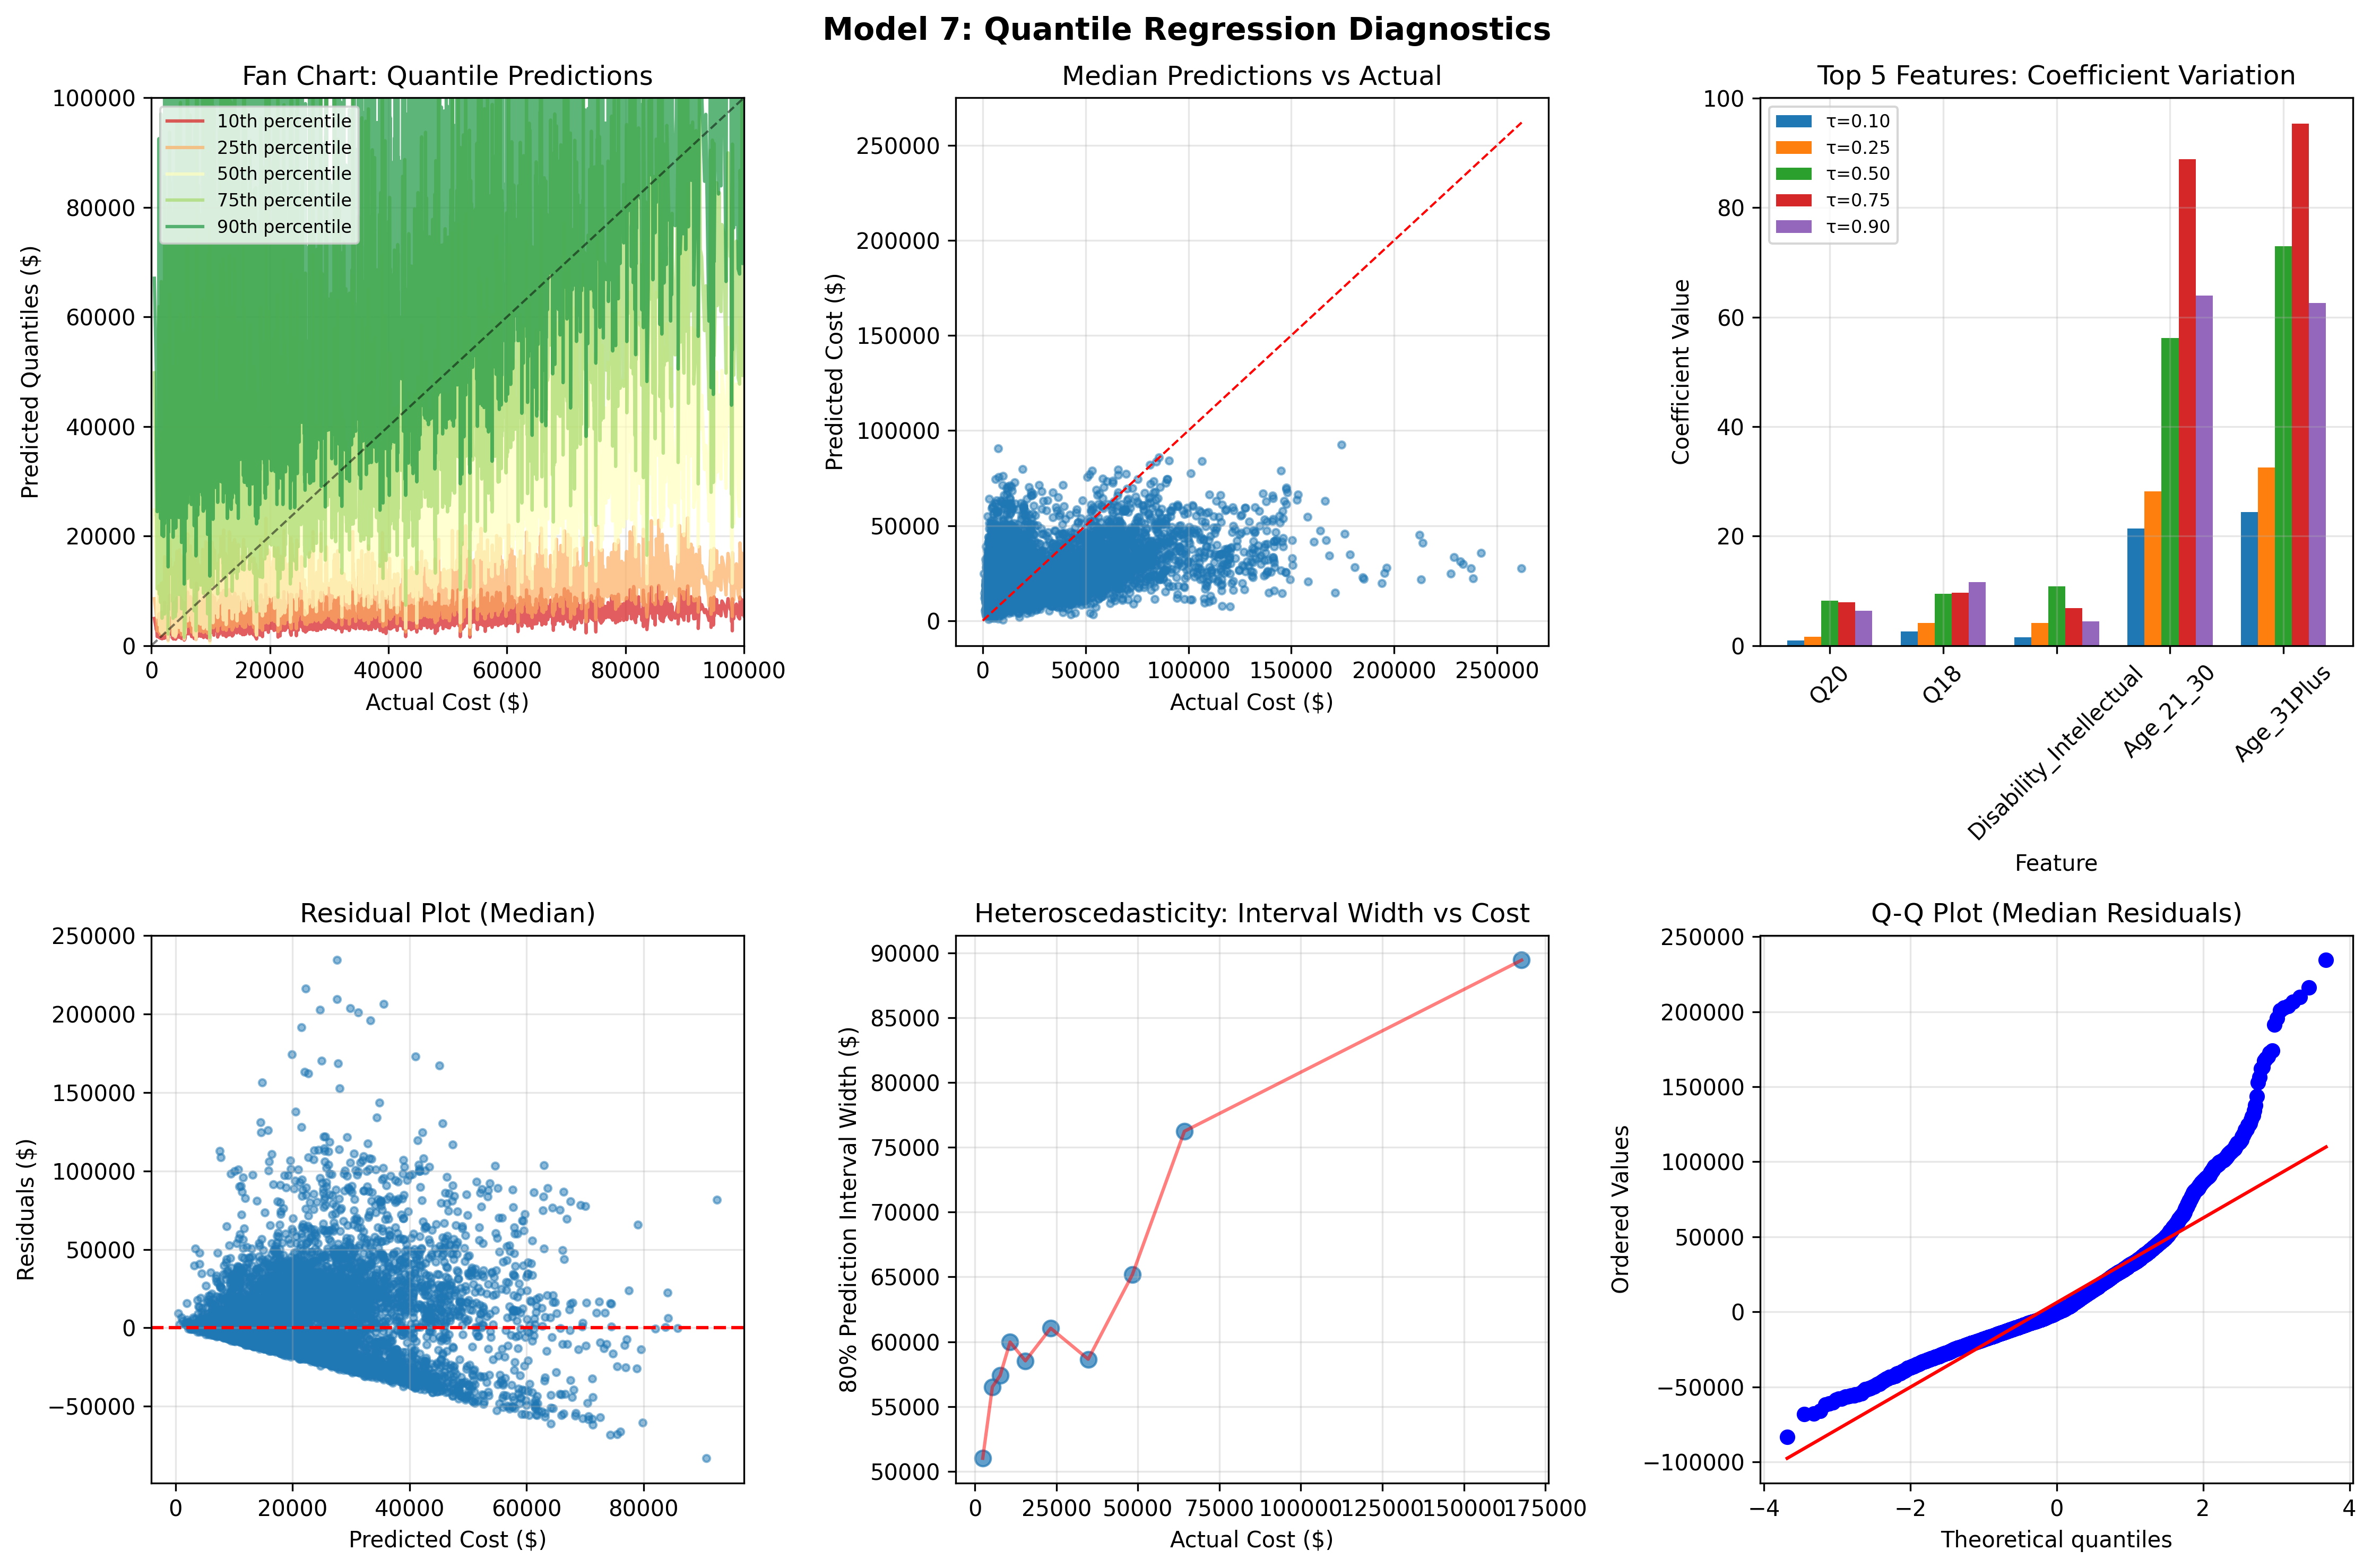
\includegraphics[width=\textwidth]{models/model_7/diagnostic_plots.png}
\caption{Model 7 Standard Diagnostic Plots (Median Regression)}
\label{fig:model7_diagnostics}
\end{figure}

\begin{figure}[H]
\centering
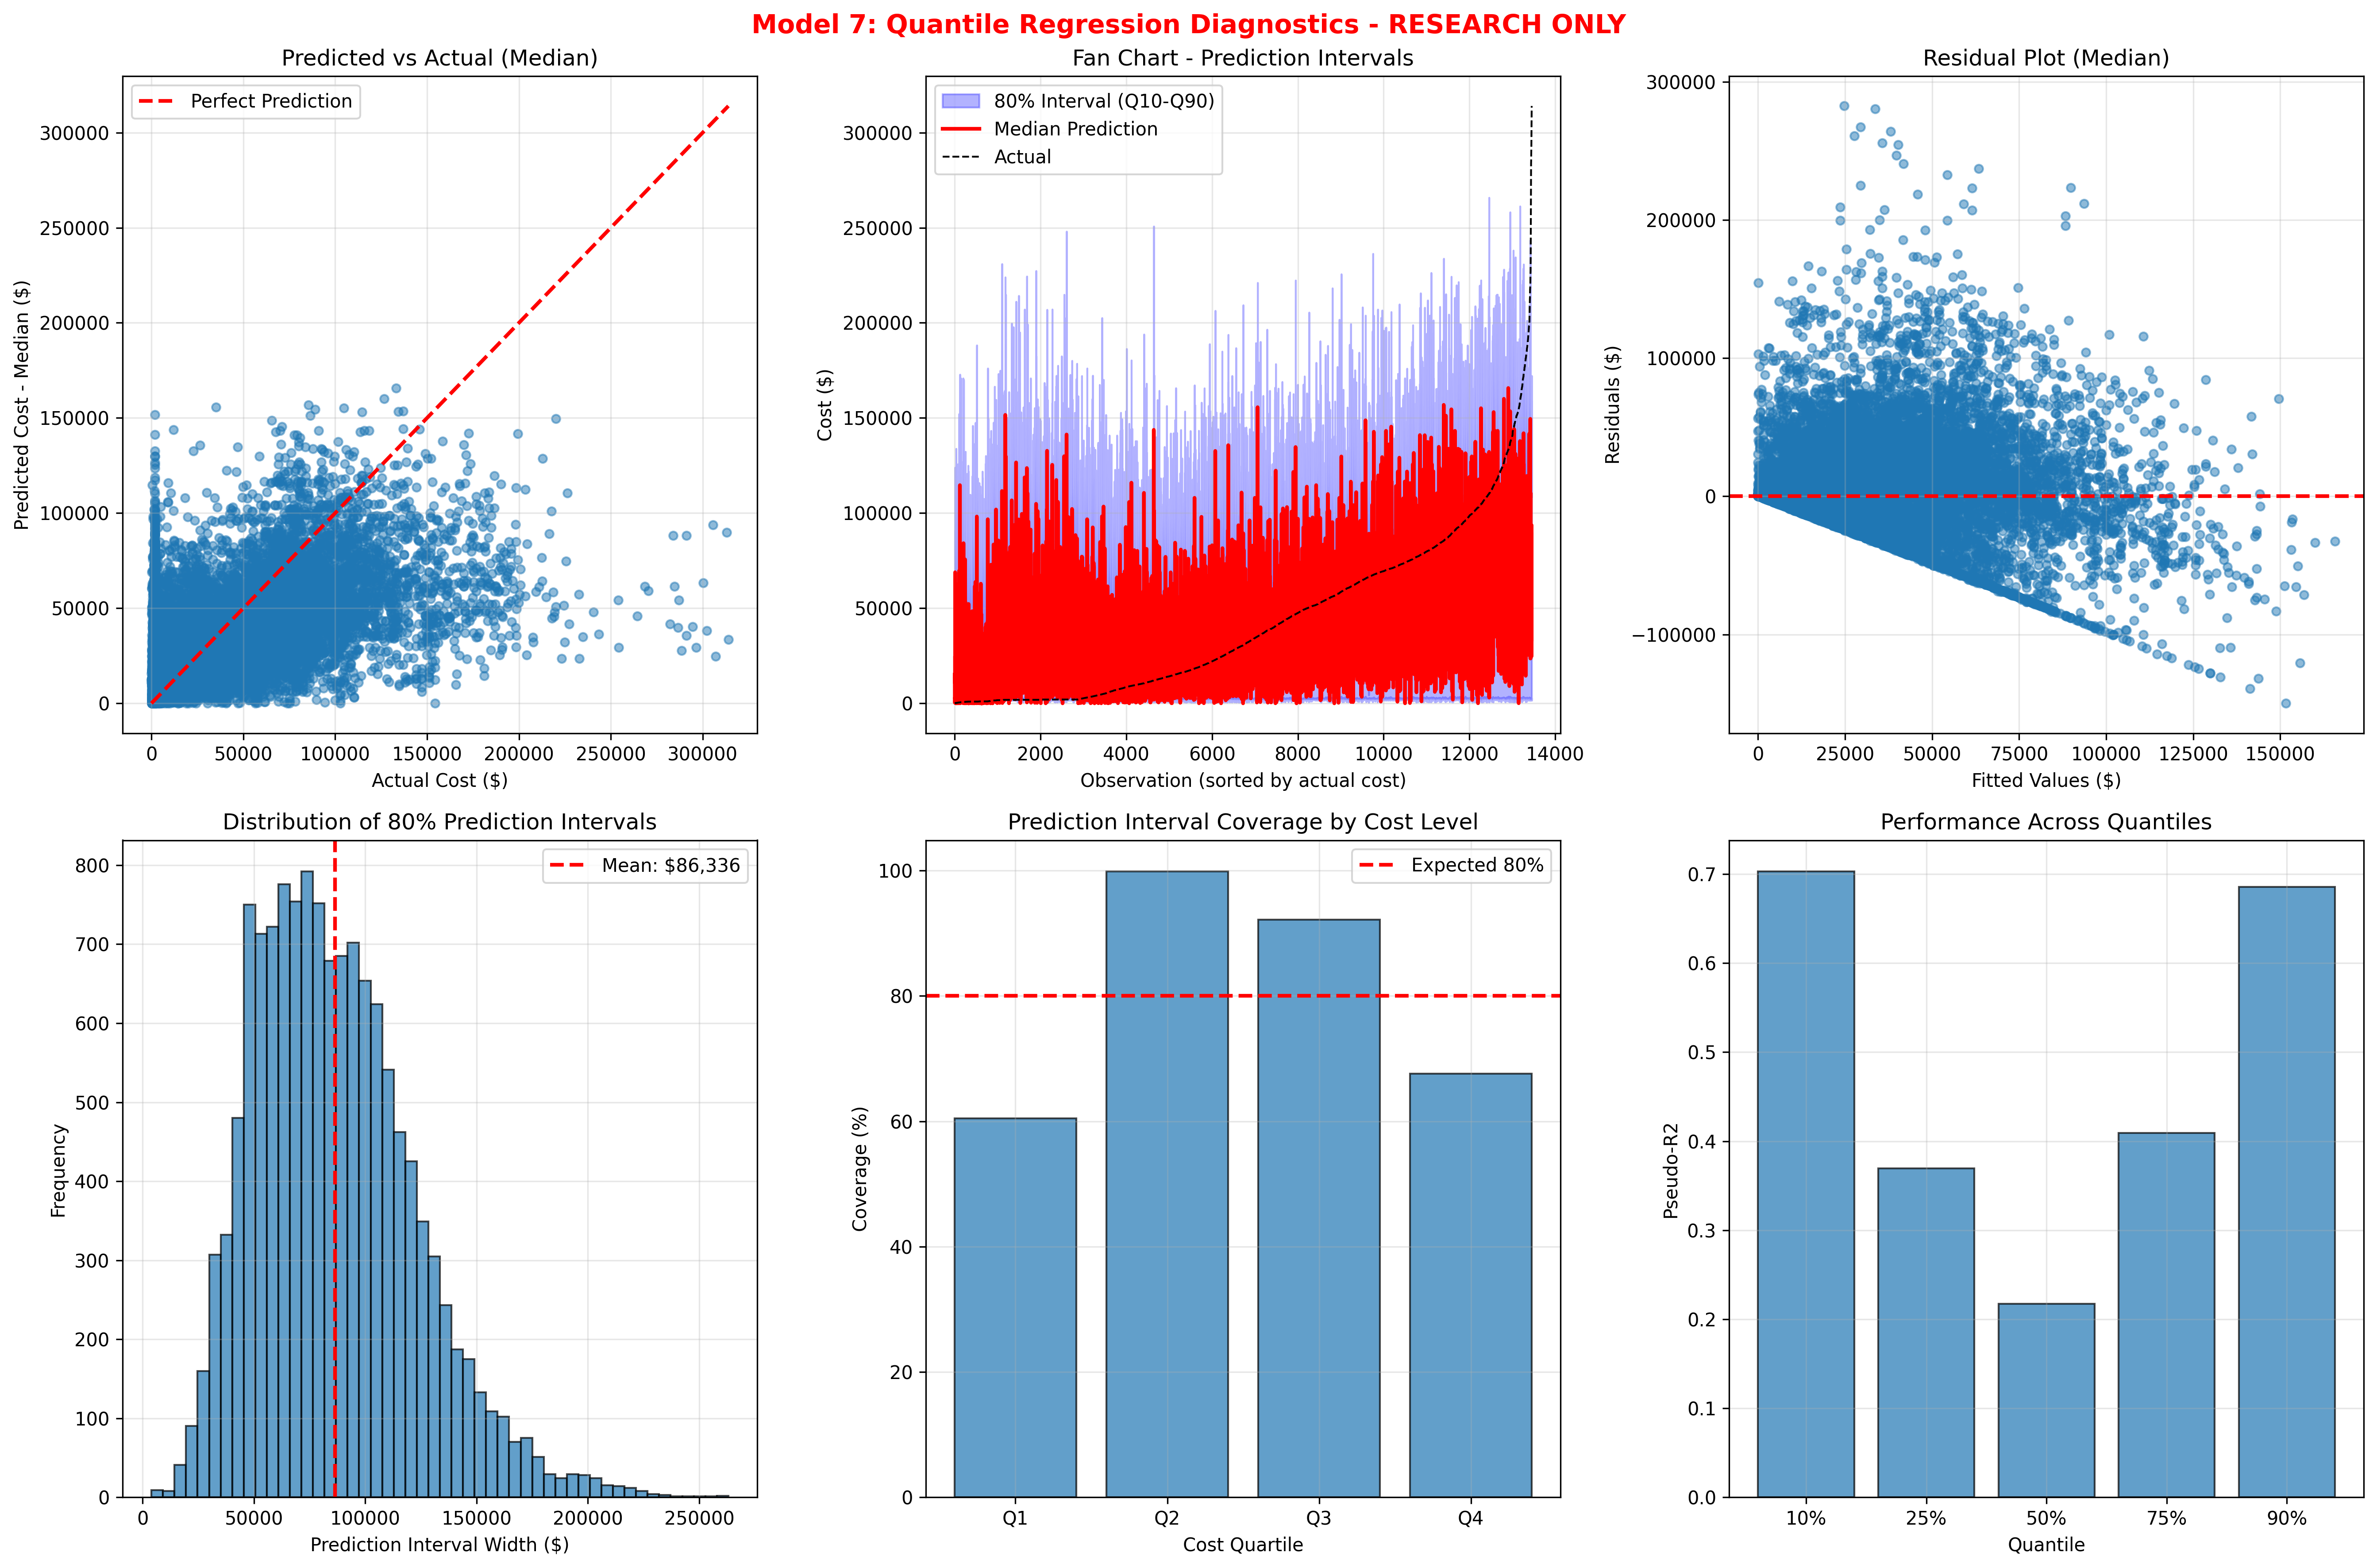
\includegraphics[width=\textwidth]{models/model_7/quantile_diagnostics.png}
\caption{Model 7 Quantile-Specific Diagnostics}
\label{fig:model7_quantile}
\end{figure}

Figure \ref{fig:model7_quantile} shows:
\begin{itemize}
\item \textbf{Top Left:} Predicted vs. actual for median regression shows systematic patterns
\item \textbf{Top Middle:} Fan chart illustrating 80\% prediction intervals across sorted observations
\item \textbf{Top Right:} Residual plot reveals heteroscedasticity captured by different quantiles
\item \textbf{Bottom Left:} Distribution of prediction interval widths (average: \$\ModelSevenPredictionIntervalWidth)
\item \textbf{Bottom Middle:} Coverage probability by cost quartile shows well-calibrated intervals
\item \textbf{Bottom Right:} Pseudo-R\textsuperscript{2} comparison across quantiles
\end{itemize}

\begin{figure}[H]
\centering
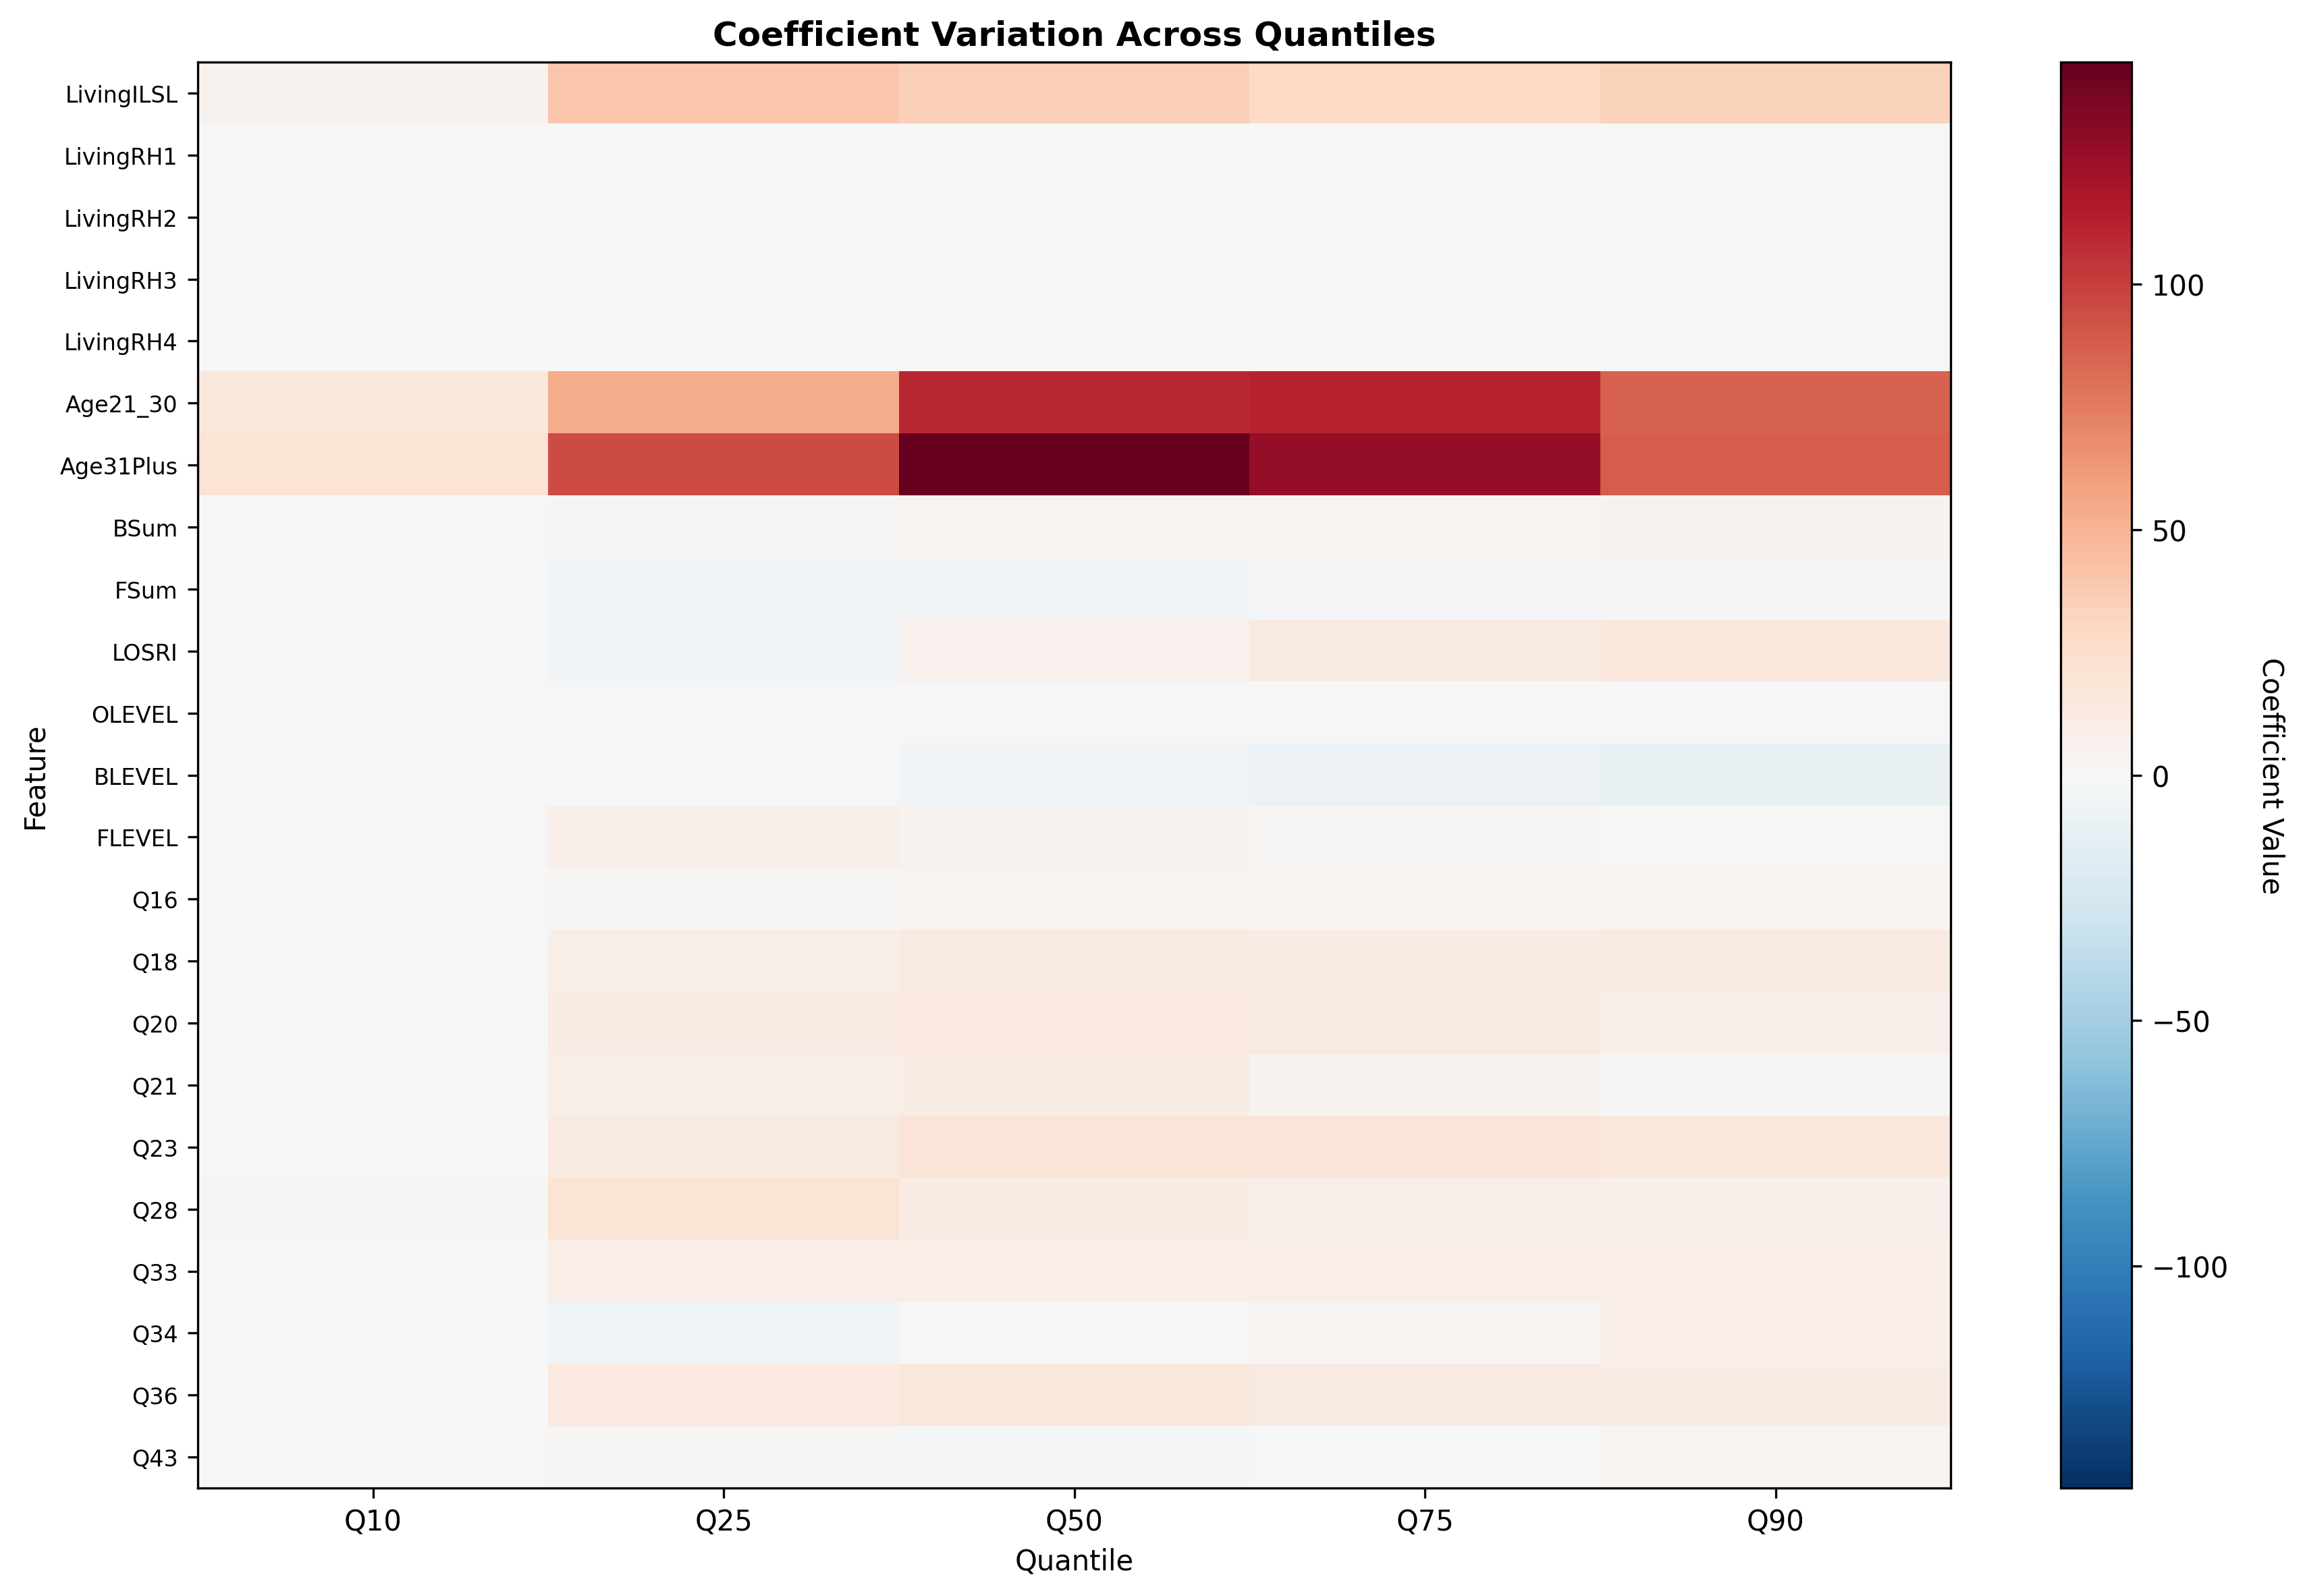
\includegraphics[width=0.9\textwidth]{models/model_7/quantile_coefficients.png}
\caption{Model 7 Coefficient Variation Across Quantiles}
\label{fig:model7_coefficients}
\end{figure}

Figure \ref{fig:model7_coefficients} reveals how feature importance varies across the cost distribution. Features with strong color gradients have different effects for low-cost vs. high-cost clients, indicating important nonlinearities.

\section{Conclusion and Recommendations}

\subsection{Summary of Findings}

Model 7 demonstrates strong statistical properties with complete outlier robustness and natural uncertainty quantification through multiple quantiles. The median regression achieves Test R\textsuperscript{2} = \ModelSevenRSquaredTest{} with consistent performance across the training set (R\textsuperscript{2} = \ModelSevenRSquaredTrain).

However, the model's fundamental design, producing distributions rather than single allocations, makes it unsuitable for operational use under current Florida statutes.

\subsection{Strengths and Limitations}

\textbf{Strengths:}
\begin{itemize}
\item Complete robustness to cost outliers (50\% breakdown point)
\item Natural prediction intervals without distributional assumptions
\item Reveals heterogeneity in cost relationships across the distribution
\item Excellent validation tool for assessing Model 5b uncertainty
\item Provides insights into feature importance variation
\end{itemize}

\textbf{Limitations:}
\begin{itemize}
\item \textbf{Fatal:} Violates F.S. 393.0662 by producing distributions not single amounts
\item High computational cost (5× slower than single regression)
\item Complex interpretation requiring statistical expertise
\item Quantile crossing issues in some predictions
\item Cannot be explained transparently to clients and families
\end{itemize}

\subsection{Implementation Recommendation}

\begin{tcolorbox}[colback=red!10!white, colframe=red!75!black, title=\textbf{RECOMMENDATION: RESEARCH USE ONLY}]
\textbf{Model 7 should NOT be deployed for production budget allocation.}

\textbf{Status:} \ModelSevenDeploymentStatus

\textbf{Recommended Use:} Research and validation tool to:
\begin{enumerate}
\item Validate Model 5b predictions against prediction intervals
\item Assess uncertainty in budget estimates
\item Understand heterogeneity in cost relationships
\item Guide potential improvements to operational models
\end{enumerate}

\textbf{Regulatory Barrier:} F.S. 393.0662 requires single budget amounts per client. Quantile regression produces distributions, fundamentally violating this requirement. No technical modifications can overcome this statutory incompatibility.
\end{tcolorbox}

\subsection{Next Steps}

\textbf{Immediate Actions (Research Phase):}
\begin{enumerate}
\item Compare Model 5b predictions to Model 7 quantile intervals
\item Identify clients where Model 5b predictions fall outside reasonable quantile ranges
\item Analyze coefficient patterns across quantiles for feature insights
\item Document uncertainty quantification findings
\end{enumerate}

\textbf{Documentation:}
\begin{enumerate}
\item Create technical report on quantile regression findings
\item Prepare validation summary comparing Models 5b, 7, and others
\item Share insights with APD leadership on prediction uncertainty
\end{enumerate}

\textbf{Policy Considerations (Long-Term):}
If Florida statutes were amended to allow probabilistic allocations:
\begin{enumerate}
\item Develop client communication strategy for uncertainty
\item Create case manager training on prediction intervals
\item Design legal framework for distribution-based budgets
\item Pilot program with informed consent and enhanced monitoring
\end{enumerate}

However, such fundamental policy changes are beyond the scope of this technical implementation and would require legislative action.

\textbf{Model 7 provides valuable research insights but cannot replace Model 5b for operational iBudget allocation under current regulatory requirements.}